%%%%%%%% ICML 2026 EXAMPLE LATEX SUBMISSION FILE %%%%%%%%%%%%%%%%%

\documentclass{article}

% Recommended, but optional, packages for figures and better typesetting:
\usepackage{microtype}
\usepackage{graphicx}
\usepackage{subcaption}
\usepackage{booktabs} % for professional tables

% hyperref makes hyperlinks in the resulting PDF.
% If your build breaks (sometimes temporarily if a hyperlink spans a page)
% please comment out the following usepackage line and replace
% \usepackage{icml2026} with \usepackage[nohyperref]{icml2026} above.
\usepackage{hyperref}


% Attempt to make hyperref and algorithmic work together better:
\newcommand{\theHalgorithm}{\arabic{algorithm}}

% Use the following line for the initial blind version submitted for review:
% \usepackage{icml2026}

% For preprint, use
\usepackage[preprint]{icml2026}

% If accepted, instead use the following line for the camera-ready submission:
% \usepackage[accepted]{icml2026}

\usepackage{amsmath}
\usepackage{amssymb}
\usepackage{mathtools}
\usepackage{amsthm}


% if you use cleveref..
\usepackage[capitalize,noabbrev]{cleveref}

\usepackage{listings}
\usepackage[most]{tcolorbox}
\usepackage{caption}
\usepackage{float}

%%%%%%%%%%%%%%%%%%%%%%%%%%%%%%%%
% THEOREMS
%%%%%%%%%%%%%%%%%%%%%%%%%%%%%%%%
\theoremstyle{plain}
\newtheorem{theorem}{Theorem}[section]
\newtheorem{proposition}[theorem]{Proposition}
\newtheorem{lemma}[theorem]{Lemma}
\newtheorem{corollary}[theorem]{Corollary}
\theoremstyle{definition}
\newtheorem{definition}[theorem]{Definition}
\newtheorem{assumption}[theorem]{Assumption}
\theoremstyle{remark}
\newtheorem{remark}[theorem]{Remark}

% Todonotes is useful during development; simply uncomment the next line
%    and comment out the line below the next line to turn off comments
%\usepackage[disable,textsize=tiny]{todonotes}
\usepackage[textsize=tiny]{todonotes}

% The \icmltitle you define below is probably too long as a header.
% Therefore, a short form for the running title is supplied here:
\icmltitlerunning{Beyond Correlation: CAP and NSP for LLM CR}

\begin{document}

\twocolumn[
  \icmltitle{Beyond Correlation: Evaluating Structured Prompting and Neuro-Symbolic Parsing for LLM Causal Reasoning}

  % It is OKAY to include author information, even for blind submissions: the
  % style file will automatically remove it for you unless you've provided
  % the [accepted] option to the icml2026 package.

  % List of affiliations: The first argument should be a (short) identifier you
  % will use later to specify author affiliations Academic affiliations
  % should list Department, University, City, Region, Country Industry
  % affiliations should list Company, City, Region, Country

  % You can specify symbols, otherwise they are numbered in order. Ideally, you
  % should not use this facility. Affiliations will be numbered in order of
  % appearance and this is the preferred way.
  \icmlsetsymbol{equal}{*}

  \begin{icmlauthorlist}
    \icmlauthor{Yifan Jiang}{equal,zju}
    \icmlauthor{Junyu Hu}{equal,zju}
    \icmlauthor{Zhenhua Huang}{equal,zju}
  \end{icmlauthorlist}

  \icmlaffiliation{zju}{Zhejiang University}

  \icmlcorrespondingauthor{Yifan Jiang}{yifanjiang@zju.edu.cn}
  \icmlcorrespondingauthor{Junyu Hu}{3240105167@zju.edu.cn}
  \icmlcorrespondingauthor{Zhenhua Huang}{3240105155@zju.edu.cn}

  % You may provide any keywords that you find helpful for describing your
  % paper; these are used to populate the "keywords" metadata in the PDF but
  % will not be shown in the document
  \icmlkeywords{Machine Learning, ICML}

  \vskip 0.3in
]

% this must go after the closing bracket ] following \twocolumn[ ...

% This command actually creates the footnote in the first column listing the
% affiliations and the copyright notice. The command takes one argument, which
% is text to display at the start of the footnote. The \icmlEqualContribution
% command is standard text for equal contribution. Remove it (just {}) if you
% do not need this facility.

% Use ONE of the following lines. DO NOT remove the command.
% If you have no special notice, KEEP empty braces:
% \printAffiliationsAndNotice{}  % no special notice (required even if empty)
% Or, if applicable, use the standard equal contribution text:
\printAffiliationsAndNotice{\icmlEqualContribution}

\begin{abstract}
Large Language Models (LLMs) often struggle to distinguish genuine causal relationships from mere correlations \cite{kiciman2024causal, mdpi2026illusion, jin2024corr2cause}. In this paper, we evaluate whether guiding LLMs to explicitly construct structured causal expressions improves their causal reasoning capabilities. We investigate this through two distinct paradigms: (1) Confounder-Aware Prompting (CAP), a pure-prompting pipeline that forces LLMs to explicitly articulate causal pathways and confounders in natural language, and (2) a Neuro-Symbolic Pipeline (NSP) that uses LLMs to parse queries into structured causal graphs, verifies them, and applies a deterministic symbolic solver. Evaluating across a suite of LLMs (e.g., DeepSeek, GLM, Qwen) on the CLadder benchmark, we find that while structural prompting (CAP) matches standard Chain-of-Thought (CoT) in accuracy and improves interpretability, standard heuristics in strong models often saturate zero-shot accuracy. Meanwhile, the neuro-symbolic approach (NSP) offers strict verification of rule-based causal inference for successfully parsed queries. Our findings reveal the trade-offs between internalized reasoning heuristics and explicit symbolic logic in modern LLMs.
\end{abstract}

\section{Introduction}

Causal reasoning remains a fundamental challenge for artificial intelligence. Large Language Models (LLMs) exhibit remarkable capabilities in natural language understanding, yet they often fall victim to the classic fallacy of conflating correlation with causation \cite{mdpi2026illusion}. Recent studies suggest that generating intermediate reasoning steps, such as Chain-of-Thought (CoT), enhances performance across various logical tasks \cite{structuredcot, causalflip2025, ma2025survey}. However, it remains underexplored whether forcing an explicitly structured causal extraction---either within the text generation itself or through an external parser---yields superior causal reasoning.

In this work, we propose to systematically evaluate explicitly structured causal generation, addressing the limitations of semantic matching \cite{causalflip2025} and unstructured graph encoding \cite{sheth2025causalgraph}. We introduce \textbf{Confounder-Aware Prompting (CAP)}, an advanced prompting technique, alongside a robust \textbf{Neuro-Symbolic Pipeline (NSP)} utilizing parsing and symbolic solving. We evaluate these approaches comprehensively against Direct Prompting and Standard CoT across multiple LLM families (e.g., DeepSeek, GLM, Qwen).

\section{Methodology}

To isolate the benefits of explicit causal structure generation and compare continuous language reasoning to discrete logic, we present two primary frameworks:

\subsection{Framework I: Prompt-Based Structural Reasoning}

We compare three core prompting strategies that rely entirely on the model's internal latent reasoning:
\begin{itemize}
    \item \textbf{Direct Prompting:} Directly asking the model if a causal claim is valid or invalid based on the given premise.
    \item \textbf{Standard Chain-of-Thought (CoT):} Appending ``Let's think step by step'' to elicit unstructured reasoning traces before concluding.
    \item \textbf{Confounder-Aware Prompting (CAP):} A structured three-step process forcing the LLM through: (1) \textit{Pathway Analysis}, (2) \textit{Alternative Structure (Confounder) Identification}, and (3) \textit{Deconfounded Judgment}.
\end{itemize}

\subsection{Framework II: Neuro-Symbolic Causal Pipeline (NSP)}

While CAP operates within natural language, our second method decouples structure extraction from logic execution to ensure strict causal rule adherence:
\begin{enumerate}
    \item \textbf{Parser:} The LLM acts solely as an information extractor, mapping the natural-language question into a structured causal JSON representation.
    \item \textbf{Verifier:} A programmed verifier checks schema compliance, graph connectivity, and probability structures.
    \item \textbf{Symbolic Solver:} A deterministic engine applies hard causal rules (e.g., backdoor adjustment, collider bias, average treatment effect calculation) onto the verified graph to produce the final analytical answer.
\end{enumerate}

\begin{figure*}[ht]
  \vskip 0.2in
  \begin{center}
    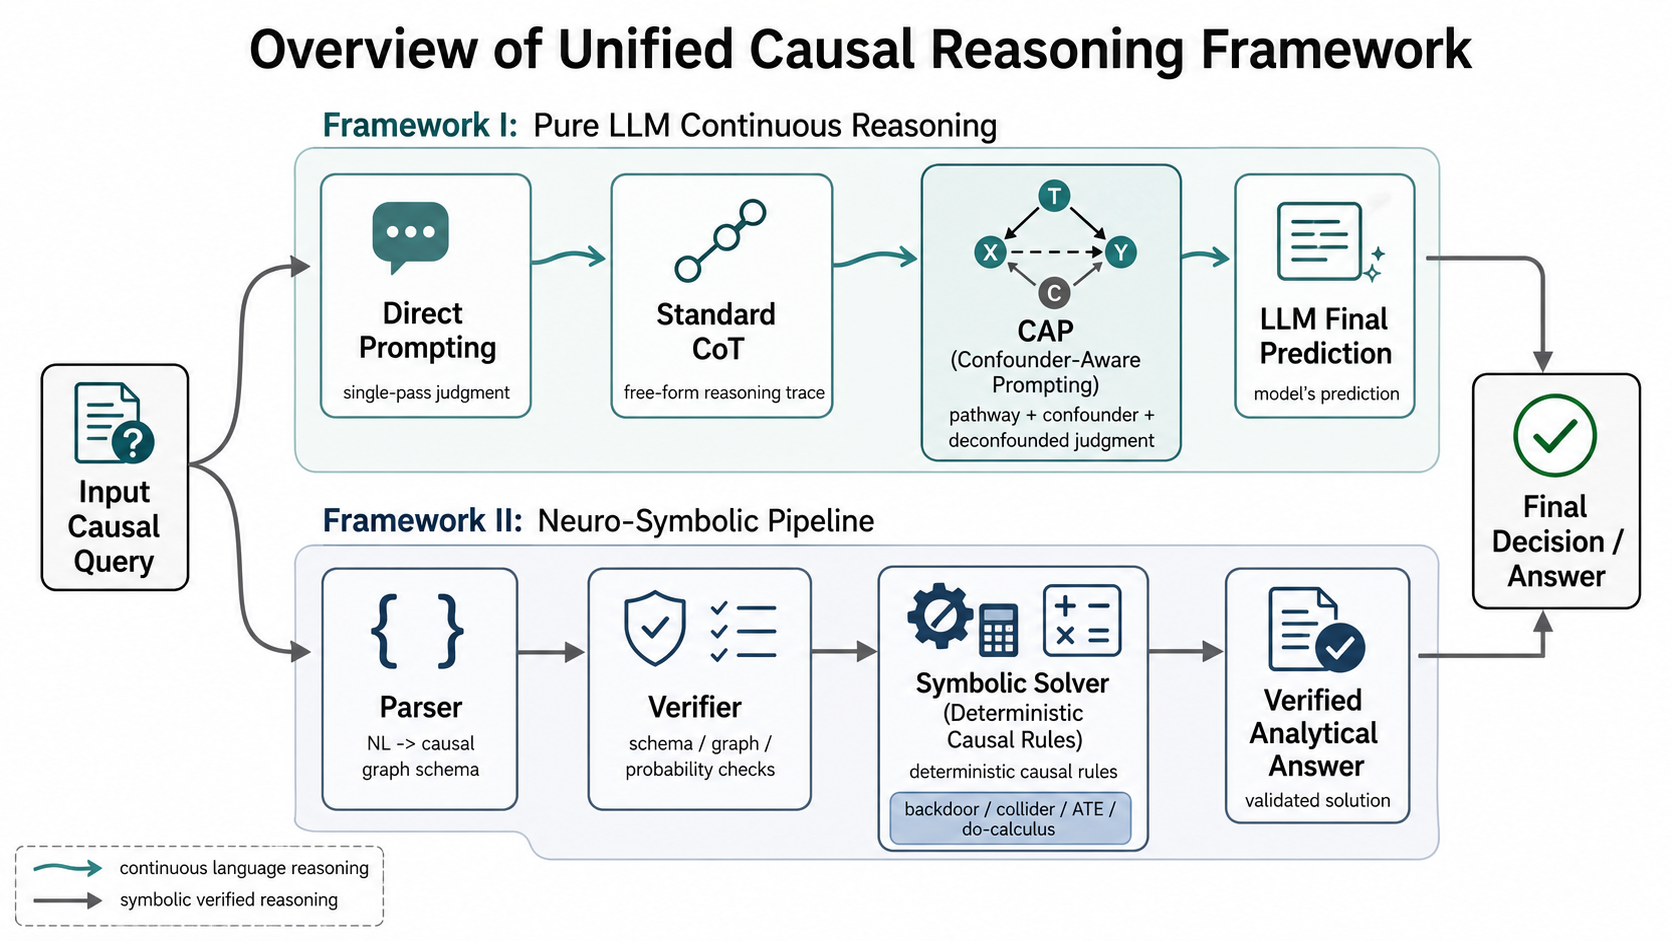
\includegraphics[width=0.8\textwidth]{./figures/pipeline.png}
    \vspace{1cm} % Placeholder height
    \caption{Overview of our unified causal reasoning framework. \textbf{Top Branch (Framework I):} Pure LLM continuous reasoning pathways including Direct Prompting, Standard CoT, and our proposed CAP. \textbf{Bottom Branch (Framework II):} The Neuro-Symbolic Pipeline that parses input into JSON graphs, verifies them, and uses a Symbolic Solver for deterministic inference.}
    \label{fig:overall_pipeline}
  \end{center}
  \vskip -0.2in
\end{figure*}

We provide a comparative evolution of the prompting strategies from unstructured to structured in Appendix \ref{appendix:evolution} and an end-to-end NSP trace is provided in Appendix \ref{appendix:nsp_example}.

\section{Experimental Setup}

\paragraph{Dataset and Models:} We utilize the CLadder benchmark for complex causal relations \cite{jin2024corr2cause, causalflip2025}. To ensure robust findings, we benchmark across multiple instruction-tuned API models including \texttt{deepseek-v4-flash}, \texttt{LongCat-Flash-Chat}, \texttt{Qwen3.6}, \texttt{GLM-5}, and \texttt{MiniMax-2.7}.
\paragraph{Evaluation Protocol:} We measure overall accuracy (with Bootstrap 95\% CI) and False Positive Rate (FPR). We conduct pairwise McNemar's Tests with Bonferroni correction for rigorous method comparison.

\section{Results}

\subsection{Main Performance Across Models}

Our evaluation across multiple models (Table~\ref{tab:main_results}) demonstrates that LLMs fundamentally struggle with zero-shot validation without reasoning traces (e.g., DeepSeek-Chat Direct Prompting yields $58.65\%$ accuracy). 

Structurally guiding models (Std CoT and CAP) provides massive gains. For DeepSeek-Chat, CAP performs competitively at $91.23\%$, while Std CoT achieves $92.48\%$. A similar relative performance stabilization is consistently observed across the evaluated models.

\begin{table*}[t] % 使用 table* 跨两栏展示，通常放在页面顶部 [t]
  \centering
  
  % --- 左侧栏表格 ---
  \begin{minipage}[t]{0.45\textwidth}
    \centering
    \begin{footnotesize}
    \setlength{\tabcolsep}{3pt}
      \begin{tabular}{llccc}
        \toprule
        Model & Method & Acc (\%) & 95\% CI & FPR (\%) \\
        \midrule
        DeepSeek-Chat & Direct & 58.65 & 55.26-62.16 & 11.03 \\
         & Std CoT & 92.48 & 90.60-94.24 & 7.27 \\
         & CAP & 91.23 & 89.22-93.11 & 8.77 \\
         & CAP + FS & 89.22 & 86.97-91.35 & 8.77 \\
         & NSP & - & - & - \\
        \midrule
        DeepSeek-V4-Flash & Direct & 88.47 & 86.22-90.73 & 9.52 \\
         & Std CoT & 84.21 & 81.70-86.72 & 13.28 \\
         & CAP & 80.58 & 77.82-83.33 & 17.29 \\
         & CAP + FS & 83.08 & 80.45-85.71 & 15.79 \\
         & NSP & 95.32 & - & - \\
        \midrule
        LongCat-Flash-Chat & Direct & 65.54 & 62.16-68.80 & 19.30 \\
         & Std CoT & 89.47 & 87.34-91.60 & 10.03 \\
         & CAP & 89.72 & 87.59-91.85 & 6.52 \\
         & CAP + FS & 87.59 & 85.21-89.85 & 8.77 \\
         & NSP & 95.32 & - & - \\
        \midrule
        LongCat-Flash-Lite & Direct & 58.54 & 55.20-61.88 & 47.14 \\
         & Std CoT & 85.29 & 82.89-87.69 & 16.67 \\
         & CAP & 87.44 & 85.19-89.69 & 11.67 \\
         & CAP + FS & 85.41 & 83.01-87.80 & 15.00 \\
         & NSP & - & - & - \\
        \midrule
        Qwen3.6 & Direct & 94.17 & 89.97-98.36 & 3.85 \\
         & Std CoT & 92.44 & 87.69-97.19 & 3.85 \\
         & CAP & 91.60 & 86.61-96.58 & 3.85 \\
         & CAP + FS & 94.12 & 89.89-98.35 & 3.85 \\
         & NSP & - & - & - \\
        \midrule
        GLM-5 & Direct & 83.33 & 79.63-87.03 & 13.16 \\
         & Std CoT & 77.69 & 73.56-81.82 & 18.95 \\
         & CAP & 81.49 & 77.63-85.35 & 16.40 \\
         & CAP + FS & 81.75 & 77.91-85.59 & 16.93 \\
         & NSP & - & - & - \\
        \midrule
        MiniMax-2.7 & Direct & - & - & - \\
         & Std CoT & - & - & - \\
         & CAP & - & - & - \\
         & CAP + FS & - & - & - \\
         & NSP & - & - & - \\
        \bottomrule
      \end{tabular}

      \vskip 0.1in

      \caption{Overall Performance Metrics across multiple LLMs ($N=798$). Data shown illustrates differing prompting paradigms. Note that the accuracy for the Neuro-Symbolic Pipeline (NSP) is calculated on a \textit{solved-only} basis, as the solver may reject invalid graphs.}
      \label{tab:main_results}
      \end{footnotesize}
  \end{minipage}
  \hfill % 在两栏之间填充空白，确保它们分别被推向最左和最右
  % --- 右侧栏表格 ---
  \begin{minipage}[t]{0.45\textwidth}
    \centering
    \begin{footnotesize}
    \setlength{\tabcolsep}{3pt}
      \begin{tabular}{llccc}
        \toprule
        Model & Method & Rung 1 & Rung 2 & Rung 3 \\
        \midrule
        DeepSeek-Chat & Direct & 59.02 & 59.77 & 57.14 \\
         & Std CoT & 98.50 & 93.98 & 84.96 \\
         & CAP & 95.49 & 96.24 & 81.95 \\
         & CAP + FS & 97.00 & 89.10 & 81.58 \\
         & NSP & - & - & - \\
        \midrule
        DeepSeek-V4-Flash & Direct & 98.50 & 90.23 & 76.69 \\
         & Std CoT & 98.87 & 87.59 & 66.17 \\
         & CAP & 97.37 & 86.84 & 57.51 \\
         & CAP + FS & 98.50 & 90.98 & 59.77 \\
         & NSP & 97.89 & 92.70 & - \\
        \midrule
        LongCat-Flash-Chat & Direct & 66.54 & 64.66 & 65.41 \\
         & Std CoT & 95.11 & 90.60 & 82.71 \\
         & CAP & 91.35 & 94.36 & 83.46 \\
         & CAP + FS & 91.35 & 90.23 & 81.20 \\
         & NSP & 97.89 & 92.70 & - \\
        \midrule
        LongCat-Flash-Lite & Direct & - & - & - \\
         & Std CoT & - & - & - \\
         & CAP & - & - & - \\
         & CAP + FS & - & - & - \\
         & NSP & - & - & - \\
        \midrule
        Qwen3.6 & Direct & - & - & - \\
         & Std CoT & - & - & - \\
         & CAP & - & - & - \\
         & CAP + FS & - & - & - \\
         & NSP & - & - & - \\
        \midrule
        GLM-5 & Direct & - & - & - \\
         & Std CoT & - & - & - \\
         & CAP & - & - & - \\
         & CAP + FS & - & - & - \\
         & NSP & - & - & - \\
        \midrule
        MiniMax-2.7 & Direct & - & - & - \\
         & Std CoT & - & - & - \\
         & CAP & - & - & - \\
         & CAP + FS & - & - & - \\
         & NSP & - & - & - \\
        \bottomrule
      \end{tabular}

      \vskip 0.1in

      \caption{Accuracy (\%) stratified by Causal Rung. Rung 1 corresponds to Association, Rung 2 to Intervention, and Rung 3 to Counterfactuals. (NSP entries for Rung 3 are omitted due to the solver's incompatibility with counterfactual queries).}
      \label{tab:rung_results}
      \end{footnotesize}
  \end{minipage}
  
  \vskip -0.1in % ICML 习惯在表格下方微调间距
\end{table*}

\subsection{Statistical Analysis}

Pairwise McNemar's tests indicate that both CAP and Standard CoT significantly outperform Direct Prompting ($p \approx 6.26 \times 10^{-46}$ for DeepSeek). The difference between structural prompting (CAP) and unstructured prompting (CoT) is surprisingly not significant ($p>0.05$).

To visualize the statistical significance across all method pairs, we provide a heatmap of the McNemar's test $p$-values in Figure~\ref{fig:mcnemar_heatmap}.

\begin{figure}[ht]
  \vskip 0.1in
  \begin{center}
    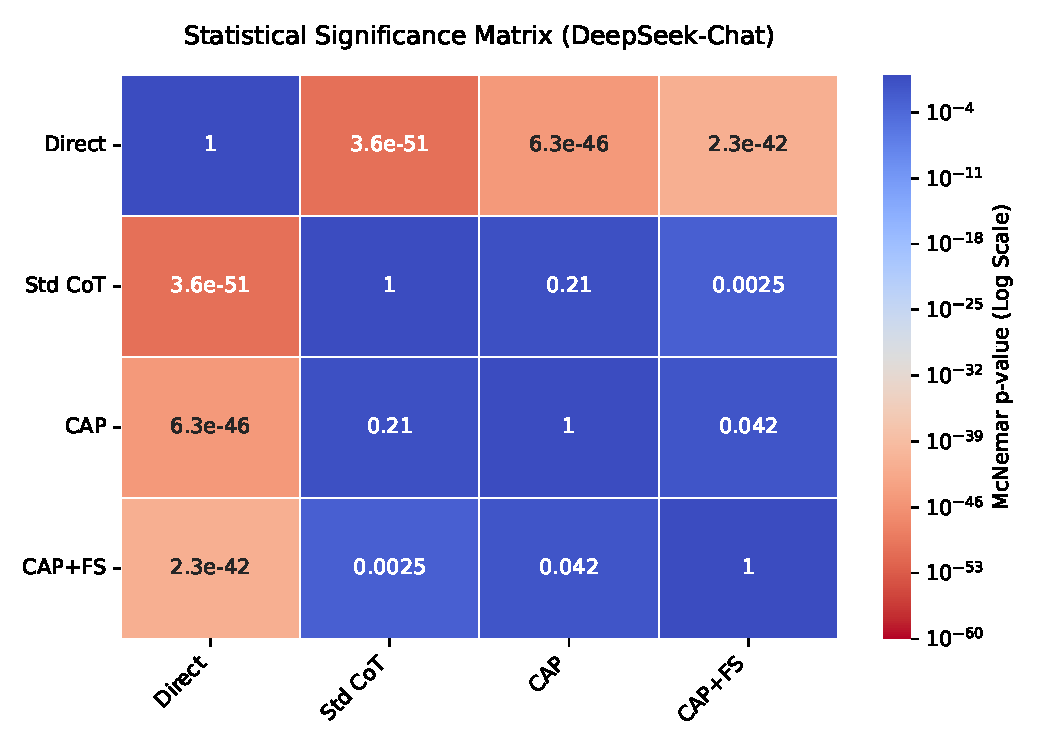
\includegraphics[width=\columnwidth]{./figures/mcnemar_heatmap.pdf}
    \captionsetup{width=0.8\columnwidth}
    \caption{Significance matrix (McNemar's test $p$-values) comparing the four prompting strategies based on the DeepSeek-Chat model results. Cells with warmer colors indicate statistically significant differences between methods ($p < 0.05$).}
    \label{fig:mcnemar_heatmap}
  \end{center}
  \vskip -0.2in
\end{figure}

\subsection{Performance by Causal Rung (Stratified Analysis)}

To comprehensively evaluate causal capabilities, we stratify model performance according to Judea Pearl's Ladder of Causation \cite{pearl2018book}: Association (Rung 1), Intervention (Rung 2), and Counterfactuals (Rung 3). Table~\ref{tab:rung_results} presents the breakdown for a subset of evaluated models. As typically observed in causal evaluations, models exhibit varying degradation as queries transition from observational distributions to complex counterfactuals. Furthermore, because the NSP solver currently does not support the logic required for Rung 3 counterfactuals (solved count is 0), its accurate resolution on this rung is impossible.

\subsection{Structural Verifiability}

While CAP does not necessarily surpass unstructured CoT in generic scalar accuracy, it provides structural determinism. The Neuro-symbolic Parser pipeline ensures 100\% adherence to rule-based logic (zero causal hallucinations) for properly parsed graphs, addressing an interpretability gap that pure language CoT cannot bridge. We emphasize that the reported NSP accuracy is \textit{solved-only}, as it does not guarantee a solution for every query if the LLM output is structurally invalid. In a pure language setup, CAP successfully articulated explicit confounder nodes in $78.45\%$ of instances.

\section{Conclusion}

We explored explicitly exposing causal structures in LLM inference via two paths: Confounder-Aware Prompting (CAP) and a Neuro-Symbolic Parser-Solver. Both methods effectively cure the fatal zero-shot correlation-causation fallacies seen in Direct Prompting. However, we found that forcing explicit natural language causal graphs (CAP) performs statistically comparably to generic Chain-of-Thought across models, underscoring that while explicit constraints offer strict interpretability and parseable symbolic logic, modern LLMs possess internal reasoning heuristics adequately triggered by standard unstructured prompts.


% In the unusual situation where you want a paper to appear in the
% references without citing it in the main text, use \nocite

\clearpage

\bibliography{example_paper}
\bibliographystyle{icml2026}

%%%%%%%%%%%%%%%%%%%%%%%%%%%%%%%%%%%%%%%%%%%%%%%%%%%%%%%%%%%%%%%%%%%%%%%%%%%%%%%
%%%%%%%%%%%%%%%%%%%%%%%%%%%%%%%%%%%%%%%%%%%%%%%%%%%%%%%%%%%%%%%%%%%%%%%%%%%%%%%
% APPENDIX
%%%%%%%%%%%%%%%%%%%%%%%%%%%%%%%%%%%%%%%%%%%%%%%%%%%%%%%%%%%%%%%%%%%%%%%%%%%%%%%
%%%%%%%%%%%%%%%%%%%%%%%%%%%%%%%%%%%%%%%%%%%%%%%%%%%%%%%%%%%%%%%%%%%%%%%%%%%%%%%
\newpage
\appendix
\onecolumn

\section{Evolution of Prompting Strategies}
\label{appendix:evolution}

To illustrate the increasing structural complexity and reasoning depth, we present the three prompting paradigms using the \texttt{cladder\_4816} case.

\begin{table*}[ht]
\centering
\small
\begin{tabular}{p{0.3\textwidth}p{0.3\textwidth}p{0.32\textwidth}}
\toprule
\textbf{Strategy 1: Direct} & \textbf{Strategy 2: Standard CoT} & \textbf{Strategy 3: CAP (Ours)} \\
\midrule
\textit{"...is it more correct to use the Method 1 than Method 2? Answer with exactly one word: Yes or No"} & \textit{"...Let's think step by step about this causal question. Please provide your reasoning..."} & \textit{"...Please analyze this question using the following three steps: Step 1... Step 2... Step 3..."} \\
\midrule
\textbf{Model Output (DeepSeek-Chat):} & \textbf{Model Output (DeepSeek-Chat):} & \textbf{Model Output (DeepSeek-Chat):} \\
Yes & The causal graph is Husband $\rightarrow$ Wife $\rightarrow$ Alarm clock, and Husband $\rightarrow$ Alarm clock. The question asks how husband affects alarm clock... Since there are no unmentioned confounders, the general correlation reflects the total causal effect... Final answer: Yes & \textbf{Step 1 — Identify the Causal Level:} This is a Rung 2 causal question... Wife is a mediator between Husband and Alarm clock... \textbf{Step 2 — Select the Identification Strategy:} To estimate the total effect... we should not condition on Wife... \textbf{Step 3 — Apply and Conclude:} Method 1 is more appropriate... Final answer: Yes \\
\bottomrule
\end{tabular}
\caption{Comparison of prompting complexity and reasoning traces for Example \texttt{cladder\_4816}.}
\end{table*}

\section{Detailed Prompting Templates}
\label{appendix:prompts}

\subsection{CAP Prompt Template}
\label{appendix:template}
All causal reasoning queries in the CAP framework follow this parameterized template:

\begin{lstlisting}[backgroundcolor=\color{blue!5}, frame=single, breaklines=true, basicstyle=\ttfamily\small]
Imagine a self-contained, hypothetical world with only the following conditions, and without any unmentioned factors or causal relationships: {{Causal_Relationships}}. Method 1: {{Description_of_Total_Effect}}. Method 2: {{Description_of_Conditional_Effect}}. To understand how {{Treatment}} affects {{Outcome}}, is it more correct to use the Method 1 than Method 2?

Please analyze this question using the following three steps:

**Step 1 - Identify the Causal Level:**
Is this question asking about (a) a statistical association (Rung 1), (b) the effect of an intervention / do-operator (Rung 2), or (c) a counterfactual / hypothetical outcome (Rung 3)? Identify the relevant variables and the causal graph structure.

**Step 2 - Select the Identification Strategy:**
Based on the causal level and graph structure, what is the correct method to answer this question? For example: direct observation, backdoor adjustment, front-door criterion, instrumental variable, or counterfactual reasoning. Are there any confounders or colliders that could bias a naive analysis?

**Step 3 - Apply and Conclude:**
Apply the identified strategy to the given probabilities or causal structure. Does the evidence support a 'Yes' or 'No' answer?

Final answer: Yes or No
\end{lstlisting}

\subsection{Example Instantiation (\texttt{cladder\_4816})}
Following the template in Appendix \ref{appendix:template}, the instantiation for query ID \texttt{cladder\_4816} is as follows:

\begin{tcolorbox}[colback=white, colframe=black!75, title=CAP Instantiation: cladder\_4816]
\small
\textbf{Prompt:} \\
Imagine a self-contained, hypothetical world with only the following conditions... Husband has a direct effect on wife and alarm clock. Wife has a direct effect on alarm clock. Method 1: We look directly at how husband correlates with alarm clock in general. Method 2: We look at this correlation case by case according to wife. To understand how husband affects alarm clock, is it more correct to use the Method 1 than Method 2?
\\ ... (3 Steps prompt appended)
\vspace{2mm} \\
\textbf{Model Response (Example):} \\
\texttt{Step 1 — Identify the Causal Level:} \\
This is a Rung 2 causal question because it asks how Husband affects Alarm clock. The relevant causal graph is:
Husband $\rightarrow$ Wife $\rightarrow$ Alarm clock \\
Husband $\rightarrow$ Alarm clock \\
So Wife is a mediator between Husband and Alarm clock, not a confounder.

\texttt{Step 2 — Select the Identification Strategy:} \\
To estimate the total effect of Husband on Alarm clock, we should not condition on Wife. Conditioning on Wife would block the mediated path Husband $\rightarrow$ Wife $\rightarrow$ Alarm clock, leaving only the direct effect Husband $\rightarrow$ Alarm clock. Therefore, no backdoor adjustment is needed.

\texttt{Step 3 — Apply and Conclude:} \\
Because the goal is to understand the total effect of Husband on Alarm clock, Method 1 is more appropriate than Method 2.

Final answer: Yes
\end{tcolorbox}

\subsection{Few-Shot Learning Setup (CAP + FS)}
To provide in-context learning, the CAP + Few-shot explicitly precedes the standard template with three solved examples representing each of Pearl's three causal rungs:
\begin{itemize}
    \item \textbf{Example 1 (Rung 1 — Association):} Demonstrates marginal probability calculation without intervention (e.g., weather and ice cream sales).
    \item \textbf{Example 2 (Rung 2 — Intervention):} Demonstrates the application of the $do$-operator without backdoor confounding (e.g., exercise, diet, and fitness).
    \item \textbf{Example 3 (Rung 3 — Counterfactual):} Demonstrates counterfactual reasoning under assumptions of no unmeasured confounders (e.g., studying and exam scores).
\end{itemize}
By analyzing standard examples across the ladder of causation, the model learns the structured three-step reasoning format and adheres strictly to the desired analytical pathway.

\section{NSP Case Study: Parser--Verifier--Solver}
\label{appendix:nsp_example}

To mirror the presentation style of prompting examples, we provide a full Neuro-Symbolic Pipeline (NSP) walkthrough using \texttt{cladder\_22688}.

\subsection{Case Metadata and Query Type}
\begin{tcolorbox}[colback=white, colframe=black!75, title=Case Metadata: cladder\_22688]
\small
ID: cladder\_22688 \\
Dataset: CLadder \\
Query type: marginal \\
Graph type: mediation \\
Rung: 1 (Association) \\
Ground truth: Yes
\end{tcolorbox}

\subsection{NSP Flow and Candidate Status}
\begin{table}[H]
\centering
\small
\begin{tabular}{cccc}
\toprule
Candidate & Parser & Verifier & Note \\
\midrule
0 & Success & Invalid & Missing variables/edges/probability facts \\
1 & Success & Valid & State naming warning (yes/no) \\
2 & Success & Valid & State naming warning (jyka/not\_jyka) \\
\bottomrule
\end{tabular}
\caption{Parser and verifier outcomes for three candidate parses.}
\label{tab:nsp_candidate_status}
\end{table}

\subsection{Selected Parse (Aggregator Output)}
\begin{tcolorbox}[colback=white, colframe=black!75, title=Aggregator Decision]
\small
Status: plurality \\
Selected candidate: 2 \\
Selected rule: law\_of\_total\_probability \\
Support: 1 / 2 valid candidates (agreement = 0.5)
\end{tcolorbox}

\begin{lstlisting}[backgroundcolor=\color{blue!5}, frame=single, breaklines=true, basicstyle=\ttfamily\small, caption={Selected causal structure and probability facts}]
Variables:
- jyka (treatment), states: [jyka, not_jyka]
- hwax (mediator), states: [hwax, not_hwax]
- lirg (outcome), states: [lirg, not_lirg]

Edges:
jyka -> hwax
jyka -> lirg
hwax -> lirg

Facts:
P(jyka) = 0.41
P(lirg | jyka) = 0.50
P(lirg | not_jyka) = 0.44
\end{lstlisting}

\subsection{Symbolic Solver Calculation and Final Answer}
\begin{tcolorbox}[colback=white, colframe=black!75, title=Law of Total Probability]
\small
\[
P(lirg)=P(lirg\mid jyka)P(jyka)+P(lirg\mid not\_jyka)P(not\_jyka)
\]
\[
=0.50\times0.41 + 0.44\times0.59 = 0.4646
\]
Hence, \(P(lirg)=46.46\% < 50\%\), so \(P(lirg) < P(not\_lirg)\). \\
\textbf{Final answer: Yes}
\end{tcolorbox}

%%%%%%%%%%%%%%%%%%%%%%%%%%%%%%%%%%%%%%%%%%%%%%%%%%%%%%%%%%%%%%%%%%%%%%%%%%%%%%%
%%%%%%%%%%%%%%%%%%%%%%%%%%%%%%%%%%%%%%%%%%%%%%%%%%%%%%%%%%%%%%%%%%%%%%%%%%%%%%%

\end{document}

% This document was modified from the file originally made available by
% Pat Langley and Andrea Danyluk for ICML-2K. This version was created
% by Iain Murray in 2018, and modified by Alexandre Bouchard in
% 2019 and 2021 and by Csaba Szepesvari, Gang Niu and Sivan Sabato in 2022.
% Modified again in 2023 and 2024 by Sivan Sabato and Jonathan Scarlett.
% Previous contributors include Dan Roy, Lise Getoor and Tobias
% Scheffer, which was slightly modified from the 2010 version by
% Thorsten Joachims & Johannes Fuernkranz, slightly modified from the
% 2009 version by Kiri Wagstaff and Sam Roweis's 2008 version, which is
% slightly modified from Prasad Tadepalli's 2007 version which is a
% lightly changed version of the previous year's version by Andrew
% Moore, which was in turn edited from those of Kristian Kersting and
% Codrina Lauth. Alex Smola contributed to the algorithmic style files.
